% !TEX program = xelatex
% ============================================================
%  Deep Generative Models — Chapter 5: Diffusion Models and the Score-SDE Framework
% ============================================================

\documentclass[11pt,a4paper]{article}

% ============================================================
% §0  Fonts and page layout
% ============================================================
\IfFileExists{ctex.sty}{\usepackage[fontset=fandol]{ctex}}{}
\IfFileExists{geometry.sty}{%
  \usepackage[margin=2.5cm]{geometry}
}{%
  \PackageWarning{geometry}{geometry package not found; using default A4 margins.}%
}
\usepackage{microtype}
\linespread{1.08}
\setlength{\parskip}{0.32em}
\setlength{\parindent}{2em}

% ============================================================
% §1  Packages
% ============================================================
\usepackage{amsmath,amssymb,amsthm}
\renewcommand{\proofname}{Proof}
\usepackage{mathtools}
\usepackage{booktabs}
\usepackage{tabularx}
\usepackage{enumitem}
\usepackage{tikz}
\usetikzlibrary{arrows.meta,calc,positioning}
\usepackage[dvipsnames]{xcolor}
\usepackage[most]{tcolorbox}
\usepackage{titlesec}
\setlist[itemize]{itemsep=0.2em,topsep=0.3em,leftmargin=1.4em}
\setlist[enumerate]{itemsep=0.2em,topsep=0.3em,leftmargin=1.6em}

% ============================================================
% §2  Colors and hyperlinks
% ============================================================
\definecolor{mydarkblue}{rgb}{0.0,0.08,0.45}
\definecolor{highlight}{HTML}{FCD66F}
\definecolor{warning}{HTML}{E57373}
\definecolor{info}{HTML}{4DB6AC}
\definecolor{softblue}{HTML}{EAF2FF}
\definecolor{softgray}{HTML}{F5F5F7}

\newcommand{\tlight}[1]{\textcolor{warning}{#1}}
\newcommand{\tinfo}[1]{\textcolor{info}{#1}}

\usepackage{hyperref}
\hypersetup{
  colorlinks=true,
  linkcolor=mydarkblue,
  citecolor=mydarkblue,
  urlcolor=mydarkblue
}

% ============================================================
% §3  Mathematical notation
% ============================================================
\renewcommand{\d}{\mathrm{d}}
\newcommand{\R}{\mathbb{R}}
\newcommand{\E}{\mathbb{E}}
\newcommand{\cN}{\mathcal{N}}
\newcommand{\pdata}{p_{\mathrm{data}}}
\newcommand{\pprior}{p_{\mathrm{prior}}}
\newcommand{\score}{\nabla_x\log p_t(x)}
\newcommand{\bW}{\overline{W}}
\DeclareMathOperator{\Var}{Var}
\DeclareMathOperator*{\argmin}{arg\,min}

% ============================================================
% §4  Section styles
% ============================================================
\titleformat{\section}
  {\large\bfseries\color{mydarkblue}}{\thesection}{0.5em}{}[\titlerule]
\titlespacing*{\section}{0pt}{1.5ex}{1ex}
\titleformat{\subsection}
  {\normalsize\bfseries}{\thesubsection}{0.5em}{}
\titlespacing*{\subsection}{0pt}{1.1ex}{0.5ex}

% ============================================================
% §5  Compact title and horizontal navigation
% ============================================================
\makeatletter
\newcommand{\makecompacttitle}{%
  \begin{tcolorbox}[
    colback=mydarkblue!5,colframe=mydarkblue!10,
    arc=3pt,boxrule=0.5pt,
    left=5pt,right=5pt,top=5pt,bottom=5pt
  ]
    {\large\bfseries\@title}\hfill{\small\@author}\\[-2pt]
    {\tiny\color{gray}\@date\hfill Deep Generative Models Notes}
  \end{tcolorbox}
  \vspace{-1em}
}
\makeatother

\newtcolorbox{tabNavBoxSmall}[1][]{
  enhanced,
  colframe=white,colback=gray!5,coltext=black!80,
  fontupper=\sffamily\small\bfseries,
  arc=1.5mm,boxrule=0pt,bottomrule=2pt,
  left=2mm,right=2mm,top=1.5mm,bottom=1.5mm,
  #1
}

\newcommand{\horizontalTOCSDE}{%
  \begin{center}
  \begin{tcbraster}[
    raster columns=3,raster width=\linewidth,
    raster column skip=1mm,raster row skip=1mm,raster equal height
  ]
    \begin{tabNavBoxSmall}\hyperref[sec:bridge]{\ Discrete $\to$ Continuous}\end{tabNavBoxSmall}
    \begin{tabNavBoxSmall}\hyperref[sec:forward]{\ Forward SDE}\end{tabNavBoxSmall}
    \begin{tabNavBoxSmall}\hyperref[sec:marginals]{\ Gaussian Marginals}\end{tabNavBoxSmall}
    \begin{tabNavBoxSmall}\hyperref[sec:reverse]{\ Reverse-Time SDE}\end{tabNavBoxSmall}
    \begin{tabNavBoxSmall}\hyperref[sec:score]{\ Score Learning}\end{tabNavBoxSmall}
    \begin{tabNavBoxSmall}\hyperref[sec:sampling]{\ Sampling}\end{tabNavBoxSmall}
  \end{tcbraster}
  \vspace{-2.5pt}%
  \noindent\textcolor{gray!30}{\rule{\linewidth}{1pt}}
  \end{center}
  \vspace{0.8em}
}

% ============================================================
% §6  Boxed theorem environments
% ============================================================
\tcbset{
  mytheo/.style={
    enhanced,breakable,
    colback=#1!5!white,colframe=#1!70!black,
    coltitle=white,fonttitle=\bfseries\small,
    boxrule=0.6pt,arc=3pt,
    left=5pt,right=5pt,top=10pt,bottom=5pt,
    attach boxed title to top left={yshift*=-\tcboxedtitleheight/2,xshift=2mm},
    boxed title style={
      colback=#1!80!black,colframe=#1!80!black,
      boxrule=0pt,arc=2pt
    }
  }
}

\newtcbtheorem[auto counter]             {definition} {Definition}{mytheo=NavyBlue}{def}
\newtcbtheorem[use counter from=definition]{theorem}  {Theorem}{mytheo=WildStrawberry}{thm}
\newtcbtheorem[use counter from=definition]{proposition}{Proposition}{mytheo=JungleGreen}{prop}
\newtcbtheorem[use counter from=definition]{example}  {Example}{mytheo=YellowOrange}{ex}
\newtcbtheorem[use counter from=definition]{remark}   {Remark}{mytheo=Periwinkle}{rem}

\tcolorboxenvironment{proof}{
  blanker,breakable,left=4pt,right=4pt,top=3pt,bottom=3pt,
  borderline west={2pt}{0pt}{gray!50}
}

% ============================================================
% §7  Body
% ============================================================
\title{Chapter 5: Diffusion Models --- Score-Based SDE Framework}
\author{}
\date{2026-07-16}

\begin{document}

\makecompacttitle
\horizontalTOCSDE

\begin{center}
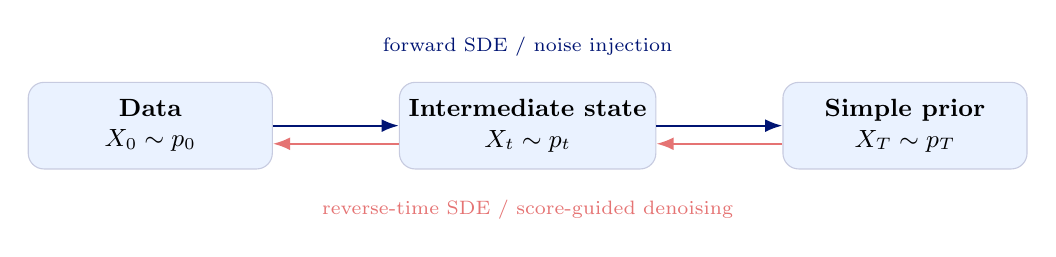
\begin{tikzpicture}[
  node distance=10mm and 16mm,
  card/.style={draw=mydarkblue!22,fill=softblue,rounded corners=2mm,
               minimum width=31mm,minimum height=11mm,align=center,font=\small\bfseries},
  arr/.style={-{Latex[length=2.2mm]},thick,mydarkblue},
  rev/.style={-{Latex[length=2.2mm]},thick,warning}
]
  \node[card] (data) {Data\\$X_0\sim p_0$};
  \node[card,right=of data] (mid) {Intermediate state\\$X_t\sim p_t$};
  \node[card,right=of mid] (noise) {Simple prior\\$X_T\sim p_T$};
  \draw[arr] (data.east) -- (mid.west);
  \draw[arr] (mid.east) -- (noise.west);
  \node[above=2mm of mid,font=\scriptsize,text=mydarkblue]
    {forward SDE / noise injection};
  \draw[rev] ([yshift=-2.3mm]noise.west) --
    ([yshift=-2.3mm]mid.east);
  \draw[rev] ([yshift=-2.3mm]mid.west) -- ([yshift=-2.3mm]data.east);
  \node[below=2.6mm of mid,font=\scriptsize,text=warning]
    {reverse-time SDE / score-guided denoising};
\end{tikzpicture}
\end{center}

The score-SDE viewpoint places noise-conditional score networks (NCSN) and
denoising diffusion probabilistic models (DDPM) inside one continuous-time
framework.  A fixed forward stochastic differential equation transports data
to a tractable noise distribution; its time reversal transports noise back to
data, provided that the time-dependent score $\score$ is known.

% ============================================================
\section{From Discrete Noise Levels to Continuous Time}\label{sec:bridge}
% ============================================================

\subsection{The common local form}

Let $0=t_0<t_1<\cdots<t_L=T$ and $\Delta t=t_{i+1}-t_i$.  Both discrete
diffusion families have, to first order, the local update
\begin{equation}\label{eq:em-local}
  X_{t+\Delta t}
  =X_t+f(X_t,t)\,\Delta t+g(t)\sqrt{\Delta t}\,Z_t,
  \qquad Z_t\sim\cN(0,I).
\end{equation}
Consequently,
\[
  p(X_{t+\Delta t}\mid X_t)
  \approx
  \cN\!\left(
    X_t+f(X_t,t)\Delta t,
    g^2(t)\Delta t\,I
  \right).
\]
Equation~\eqref{eq:em-local} is the Euler--Maruyama discretization of
\begin{equation}\label{eq:forward-sde}
  \d X_t=f(X_t,t)\,\d t+g(t)\,\d W_t,
  \qquad X_0\sim\pdata,
\end{equation}
where $W_t$ is a standard Wiener process and
$W_{t+\Delta t}-W_t\sim\cN(0,\Delta t\,I)$.

\begin{remark}{Conditioning Removes an Ambiguity}{conditioned-transition}
In the Gaussian transition above, $X_t$ is the observed conditioning value,
whereas $X_{t+\Delta t}$ is random.  Writing both symbols as if they were free
random variables obscures the meaning of the transition kernel.
\end{remark}

\subsection{NCSN / variance-exploding limit}

At noise level $\sigma_i$, NCSN uses the marginal perturbation
\[
  X_i=X_0+\sigma_i Z,
  \qquad Z\sim\cN(0,I).
\]
These marginals can be coupled as a Markov chain by injecting only the
incremental variance:
\[
  X_i=X_{i-1}
      +\sqrt{\sigma_i^2-\sigma_{i-1}^2}\,Z_i.
\]
For a differentiable increasing schedule $\sigma(t)$,
\[
  \sigma^2(t+\Delta t)-\sigma^2(t)
  \approx \frac{\d\sigma^2(t)}{\d t}\Delta t.
\]
Hence the continuous limit is the \textbf{variance-exploding (VE) SDE}
\begin{equation}\label{eq:ve-sde}
  \d X_t=\sqrt{\frac{\d\sigma^2(t)}{\d t}}\,\d W_t,
  \qquad f(x,t)=0.
\end{equation}

\subsection{DDPM / variance-preserving limit}

For DDPM, scale the discrete noise variance as
$\beta_i=\beta(t_i)\Delta t$.  Then
\[
  X_{i+1}
  =\sqrt{1-\beta(t_i)\Delta t}\,X_i
   +\sqrt{\beta(t_i)\Delta t}\,Z_i.
\]
Using $\sqrt{1-u}=1-\tfrac12u+o(u)$ gives
\[
  X_{i+1}-X_i
  =-\frac12\beta(t_i)X_i\Delta t
   +\sqrt{\beta(t_i)}\sqrt{\Delta t}\,Z_i+o(\Delta t),
\]
so the limit is the \textbf{variance-preserving (VP) SDE}
\begin{equation}\label{eq:vp-sde}
  \d X_t=-\frac12\beta(t)X_t\,\d t
          +\sqrt{\beta(t)}\,\d W_t.
\end{equation}

\begin{tcolorbox}[
  colback=softgray,colframe=mydarkblue!20,arc=2pt,boxrule=0.5pt,
  title={\bfseries Discrete-to-continuous dictionary},fonttitle=\small
]
\centering
\begin{tabularx}{\linewidth}{@{}lXX@{}}
\toprule
Family & Discrete variance per step & Continuous coefficients \\
\midrule
NCSN / VE
& $\sigma_{i+1}^2-\sigma_i^2$
& $f=0$, $g^2(t)=\frac{\d}{\d t}\sigma^2(t)$ \\
DDPM / VP
& $\beta_i=\beta(t_i)\Delta t$
& $f(x,t)=-\frac12\beta(t)x$, $g^2(t)=\beta(t)$ \\
\bottomrule
\end{tabularx}
\end{tcolorbox}

% ============================================================
\section{Forward-Time SDE: Data to Noise}\label{sec:forward}
% ============================================================

\begin{definition}{Forward Diffusion Process}{forward-diffusion}
Let the data variable $X_t$ take values in $\R^D$.  A score-based diffusion
model fixes a forward SDE on $[0,T]$
\[
  \d X_t=f(X_t,t)\,\d t+g(t)\,\d W_t,
  \qquad X_0\sim p_0=\pdata,
\]
where
\begin{itemize}[nosep]
  \item $f:\R^D\times[0,T]\to\R^D$ is the \emph{drift coefficient}, a
        vector-valued mapping specifying the deterministic part of the flow;
  \item $g:[0,T]\to\R$ is a scalar \emph{diffusion coefficient} depending only
        on time, controlling the magnitude of the injected noise (more generally
        $g$ may be matrix-valued, $g:[0,T]\to\R^{D\times D}$);
  \item $W_t$ is a $D$-dimensional standard Wiener process (Brownian motion),
        i.e.\ a process with $W_0=0$, independent Gaussian increments
        $W_{t+\Delta t}-W_t\sim\cN(0,\Delta t\,I_D)$, and almost surely
        continuous sample paths.
\end{itemize}
The terminal marginal $p_T$ is chosen to be close to a tractable prior
$\pprior$, usually an isotropic Gaussian.
\end{definition}

The forward process determines two related families of densities:
\begin{itemize}
  \item the \textbf{perturbation kernel} $p_{0t}(x_t\mid x_0)$, describing
        how a fixed clean sample becomes noisy;
  \item the \textbf{marginal density}
        \begin{equation}\label{eq:marginal-mixture}
          p_t(x_t)=\int p_{0t}(x_t\mid x_0)\,\pdata(x_0)\,\d x_0,
        \end{equation}
        obtained after averaging over clean data.
\end{itemize}

The drift $f$ may in principle be nonlinear.  In practice, the particularly
useful choice is the linear drift $f(x,t)=a(t)x$, because its perturbation
kernel is Gaussian and can be sampled exactly at any time $t$.

% ============================================================
\section{Linear SDEs and Gaussian Perturbation Kernels}\label{sec:marginals}
% ============================================================

Consider
\begin{equation}\label{eq:linear-sde}
  \d X_t=a(t)X_t\,\d t+g(t)\,\d W_t.
\end{equation}
For $0\le s\le t$, define the attenuation factor
\[
  A(t,s)\triangleq\exp\!\left(\int_s^t a(u)\,\d u\right).
\]

\begin{proposition}{Gaussian Transition of a Linear SDE}{linear-transition}
Conditioned on $X_0=x_0$, the solution of~\eqref{eq:linear-sde} is
\[
  X_t=A(t,0)x_0+\int_0^t A(t,s)g(s)\,\d W_s.
\]
Therefore
\begin{equation}\label{eq:gaussian-kernel}
  p_{0t}(x_t\mid x_0)
  =\cN\!\bigl(x_t;\,m(t)x_0,\,v(t)I\bigr),
\end{equation}
where
\begin{equation}\label{eq:mean-var}
  m(t)=A(t,0),
  \qquad
  v(t)=\int_0^t A^2(t,s)g^2(s)\,\d s.
\end{equation}
\end{proposition}

\begin{proof}
Multiplying by the integrating factor $A(0,t)$ and applying It\^o's product
rule yields the stated solution.  The stochastic integral is Gaussian with
zero mean.  It\^o isometry gives its covariance as
$\int_0^t A^2(t,s)g^2(s)\d s\,I$.
\end{proof}

Equation~\eqref{eq:gaussian-kernel} also provides the direct reparameterization
\begin{equation}\label{eq:reparam}
  X_t=m(t)X_0+\sqrt{v(t)}\,\varepsilon,
  \qquad \varepsilon\sim\cN(0,I).
\end{equation}

\subsection{The VE and VP cases}

\paragraph{VE SDE.}
For $a(t)=0$ and $g^2(t)=\frac{\d}{\d t}\sigma^2(t)$,
\[
  m(t)=1,
  \qquad
  v(t)=\sigma^2(t)-\sigma^2(0).
\]
If $\sigma(0)=0$, then
$p_{0t}(x_t\mid x_0)=\cN(x_t;x_0,\sigma^2(t)I)$.

\paragraph{VP SDE.}
For $a(t)=-\frac12\beta(t)$ and $g^2(t)=\beta(t)$, let
\[
  \alpha(t)\triangleq
  \exp\!\left(-\frac12\int_0^t\beta(u)\,\d u\right).
\]
Then
\[
  m(t)=\alpha(t),
  \qquad
  v(t)=1-\alpha^2(t),
\]
and
\begin{equation}\label{eq:vp-kernel}
  p_{0t}(x_t\mid x_0)
  =\cN\!\left(x_t;\alpha(t)x_0,
                     \bigl(1-\alpha^2(t)\bigr)I\right).
\end{equation}

\begin{remark}{When Does the Terminal Law Forget the Data?}{forget-data}
For a linear SDE, dependence on $x_0$ disappears as $m(T)\to0$.  In the VP
case, $\alpha(T)\to0$ gives $p_{0T}(x_T\mid x_0)\approx\cN(0,I)$ and therefore
$p_T\approx\cN(0,I)$ after marginalizing over $x_0$.  In the VE case the mean
remains $x_0$, but sufficiently large noise makes the data-dependent shift
negligible relative to the scale $\sigma(T)$.
\end{remark}

% ============================================================
\section{Reverse-Time Stochastic Process}\label{sec:reverse}
% ============================================================

An ODE can be reversed by a time substitution.  An SDE is subtler: diffusion
spreads probability mass, so its time reversal must include a drift that
reconstructs the changing density.  That correction is exactly the score.

\begin{theorem}{Reverse-Time SDE}{reverse-sde}
Assume the forward SDE~\eqref{eq:forward-sde} has sufficiently smooth positive
marginals $p_t$, and $g$ depends only on time.  When time runs from $T$ down to
$0$, the same family of marginals is generated by
\begin{equation}\label{eq:reverse-backward-clock}
  \d X_t
  =\Bigl[f(X_t,t)-g^2(t)\nabla_x\log p_t(X_t)\Bigr]\d t
   +g(t)\,\d\bW_t,
  \qquad \d t<0,
\end{equation}
initialized at $X_T\sim p_T$.  Here $\bW_t$ denotes Brownian motion with
respect to the decreasing-time filtration.
\end{theorem}

The sign in~\eqref{eq:reverse-backward-clock} is easy to misread because
$\d t<0$.  Introduce an increasing reverse clock $s=T-t$ and
$Y_s=X_{T-s}$.  Then the equivalent forward-in-$s$ equation is
\begin{equation}\label{eq:reverse-forward-clock}
  \d Y_s
  =\Bigl[-f(Y_s,T-s)
          +g^2(T-s)\nabla_y\log p_{T-s}(Y_s)\Bigr]\d s
   +g(T-s)\,\d W_s.
\end{equation}
Now the score term visibly points toward regions of higher density.

\begin{remark}{Why the Reverse Process Works}{reverse-intuition}
The diffusion term keeps local stochastic exploration.  The score-driven
drift compensates for that spreading and moves trajectories toward high-density
regions of the current marginal.  Early in reverse time the noise scale is
large and trajectories explore broadly; near the data endpoint the score term
restores fine structure and trajectories concentrate around the data manifold.
\end{remark}

\subsection{Connection to Langevin dynamics}

For the VE family $f=0$.  Define the time-varying temperature
\[
  \tau(s)\triangleq\frac12g^2(T-s).
\]
Equation~\eqref{eq:reverse-forward-clock} becomes
\begin{equation}\label{eq:annealed-langevin}
  \d Y_s
  =2\tau(s)\nabla_y\log p_{T-s}(Y_s)\,\d s
   +\sqrt{2\tau(s)}\,\d W_s.
\end{equation}
This has the instantaneous form of Langevin dynamics, but its target density
$p_{T-s}$ and temperature $\tau(s)$ both evolve with time.  Thus reverse
diffusion can be viewed as \emph{annealed Langevin transport}: it begins with
strong exploration and gradually shifts toward accurate reconstruction.

% ============================================================
\section{Learning the Unknown Score}\label{sec:score}
% ============================================================

The reverse SDE is exact but unusable as written because the marginal score
$\nabla_x\log p_t(x)$ is unknown.  A neural network $s_\theta(x,t)$ is trained
to approximate it at every noise level.

For the Gaussian perturbation kernel~\eqref{eq:gaussian-kernel}, the
\emph{conditional} score is available in closed form:
\begin{equation}\label{eq:conditional-score}
  \nabla_{x_t}\log p_{0t}(x_t\mid x_0)
  =-\frac{x_t-m(t)x_0}{v(t)}
  =-\frac{\varepsilon}{\sqrt{v(t)}}.
\end{equation}

\begin{proposition}{Denoising Score Matching Target}{dsm-target}
Let $t$ be sampled from a training distribution on $(0,T]$, then sample
$X_0\sim\pdata$ and $X_t\sim p_{0t}(\cdot\mid X_0)$.  For any positive weight
$\lambda(t)$, consider
\begin{equation}\label{eq:dsm-loss}
  \mathcal{L}_{\mathrm{DSM}}(\theta)
  =\E\!\left[
    \lambda(t)
    \left\|
      s_\theta(X_t,t)
      -\nabla_{x_t}\log p_{0t}(X_t\mid X_0)
    \right\|_2^2
  \right].
\end{equation}
Its pointwise population minimizer is the marginal score
$s_{\theta}^{*}(x,t)=\nabla_x\log p_t(x)$.
\end{proposition}

\begin{proof}
For fixed $(x,t)$, the least-squares minimizer is the conditional expectation
of the target given $X_t=x$.  Differentiating the mixture identity
\eqref{eq:marginal-mixture} under the integral gives
\[
  \E\!\left[
    \nabla_x\log p_{0t}(X_t\mid X_0)
    \mid X_t=x
  \right]
  =\nabla_x\log p_t(x).
\]
Thus the conditional score supplies an unbiased regression target for the
unknown marginal score.
\end{proof}

Combining~\eqref{eq:reparam} and~\eqref{eq:conditional-score}, training needs
only clean data, a random time, and standard Gaussian noise:
\[
  X_t=m(t)X_0+\sqrt{v(t)}\varepsilon,
  \qquad
  s_\theta(X_t,t)\approx-\frac{\varepsilon}{\sqrt{v(t)}}.
\]

% ============================================================
\section{Sampling with the Learned Score}\label{sec:sampling}
% ============================================================

After training, replace the unknown score in
\eqref{eq:reverse-forward-clock} with $s_\theta$.  Starting from
$Y_0\sim\pprior\approx p_T$, Euler--Maruyama with reverse-time step $\Delta s$
gives
\begin{align}\label{eq:reverse-em}
  Y_{k+1}
  ={}&Y_k+\Bigl[-f(Y_k,T-s_k)
      +g^2(T-s_k)s_\theta(Y_k,T-s_k)\Bigr]\Delta s \\
     &\quad+g(T-s_k)\sqrt{\Delta s}\,Z_k,
  \qquad Z_k\sim\cN(0,I).
\end{align}

\begin{enumerate}[label=\textbf{\arabic*.},nosep]
  \item Draw an initial sample from the terminal prior.
  \item March from noise time $T$ toward data time $0$ using
        \eqref{eq:reverse-em} (the \emph{predictor}).
  \item Optionally apply one or more Langevin correction steps at each noise
        level (the \emph{corrector}).
  \item Return the state at time $0$ as the generated sample.
\end{enumerate}

\begin{tcolorbox}[
  enhanced,colback=mydarkblue!4,colframe=mydarkblue!45,
  arc=3pt,boxrule=0.6pt,title={\bfseries Framework in one line},
  fonttitle=\small,top=2pt,bottom=2pt
]
\centering
{\small$\boxed{\begin{gathered}
    \text{discrete noise schedule}
    \longrightarrow \text{forward SDE}
    \longrightarrow \{p_t\}_{t\in[0,T]} \\
    \scriptstyle \text{learn }\nabla_x\log p_t
    \quad\Downarrow\quad \\
    \text{terminal prior}
    \longrightarrow \text{reverse-time SDE}
    \longrightarrow \text{samples}
  \end{gathered}}$}\par\smallskip
\raggedright\small
NCSN and DDPM differ chiefly in their forward drift and diffusion.  Gaussian
perturbation kernels, score matching, and a reverse-time solver then determine
the continuous model.
\end{tcolorbox}

\end{document}
